% ---
% Arquivo com a metodologia do Trabalho de Conclusão de Curso dos alunos
% Gabriel Takaoka Nishimura, Felippe Demarqui Ramos e Vivian Kimie Isuyama 
% da Escola Politécnica da Universidade de São Paulo
% ---
	% ---
	\chapter{Metodologia}\label{cap-metodologia}
	% ---
	
	Nesse capítulo são discorridas as escolhas da \texttt{norma 802.15.7}, \textit{hardware} e \texttt{software}.
	% ---
	\section{Norma IEEE 802.15.7}\label{sec-norma}
	% ---
	
	
	
	% ---
	\section{Hardware}\label{sec-hardware}
	% ---
	
	Explica as escolhas feitas de hardware.
	
	% ---
	\subsection{FPGA}\label{hard-fpga}
	% ---
	
	FPGA (Field-Programmable Gate Array) é uma tecnologia que utiliza chips de silício reprogramáveis para obter circuitos customizáveis, latência a nível de hardware\footnote{muito muito rápido} e vazão muito alta\footnote{devido ao alto grau de paralelismo}. No projeto LiCy, como o fluxo de informações é muito alto (requisito de projeto de 1Gbps), é necessário realizar múltiplos processos ao mesmo tempo para lidar com os dados:
	
	\begin{itemize}  
		\item Recebimento/Transmissão de dados
		\item Cálculo de paridade
		\item Correção de erros\footnote{apenas para recebimento}
		\item (De)codificação de dados
	\end{itemize}
	
	\begin{table}[htbp]
		\caption{\label{tab_phy1} Modos de operação da camada PHY I de Li-Fi}
		\centering
		%  trim={<left> <lower> <right> <upper>} 
		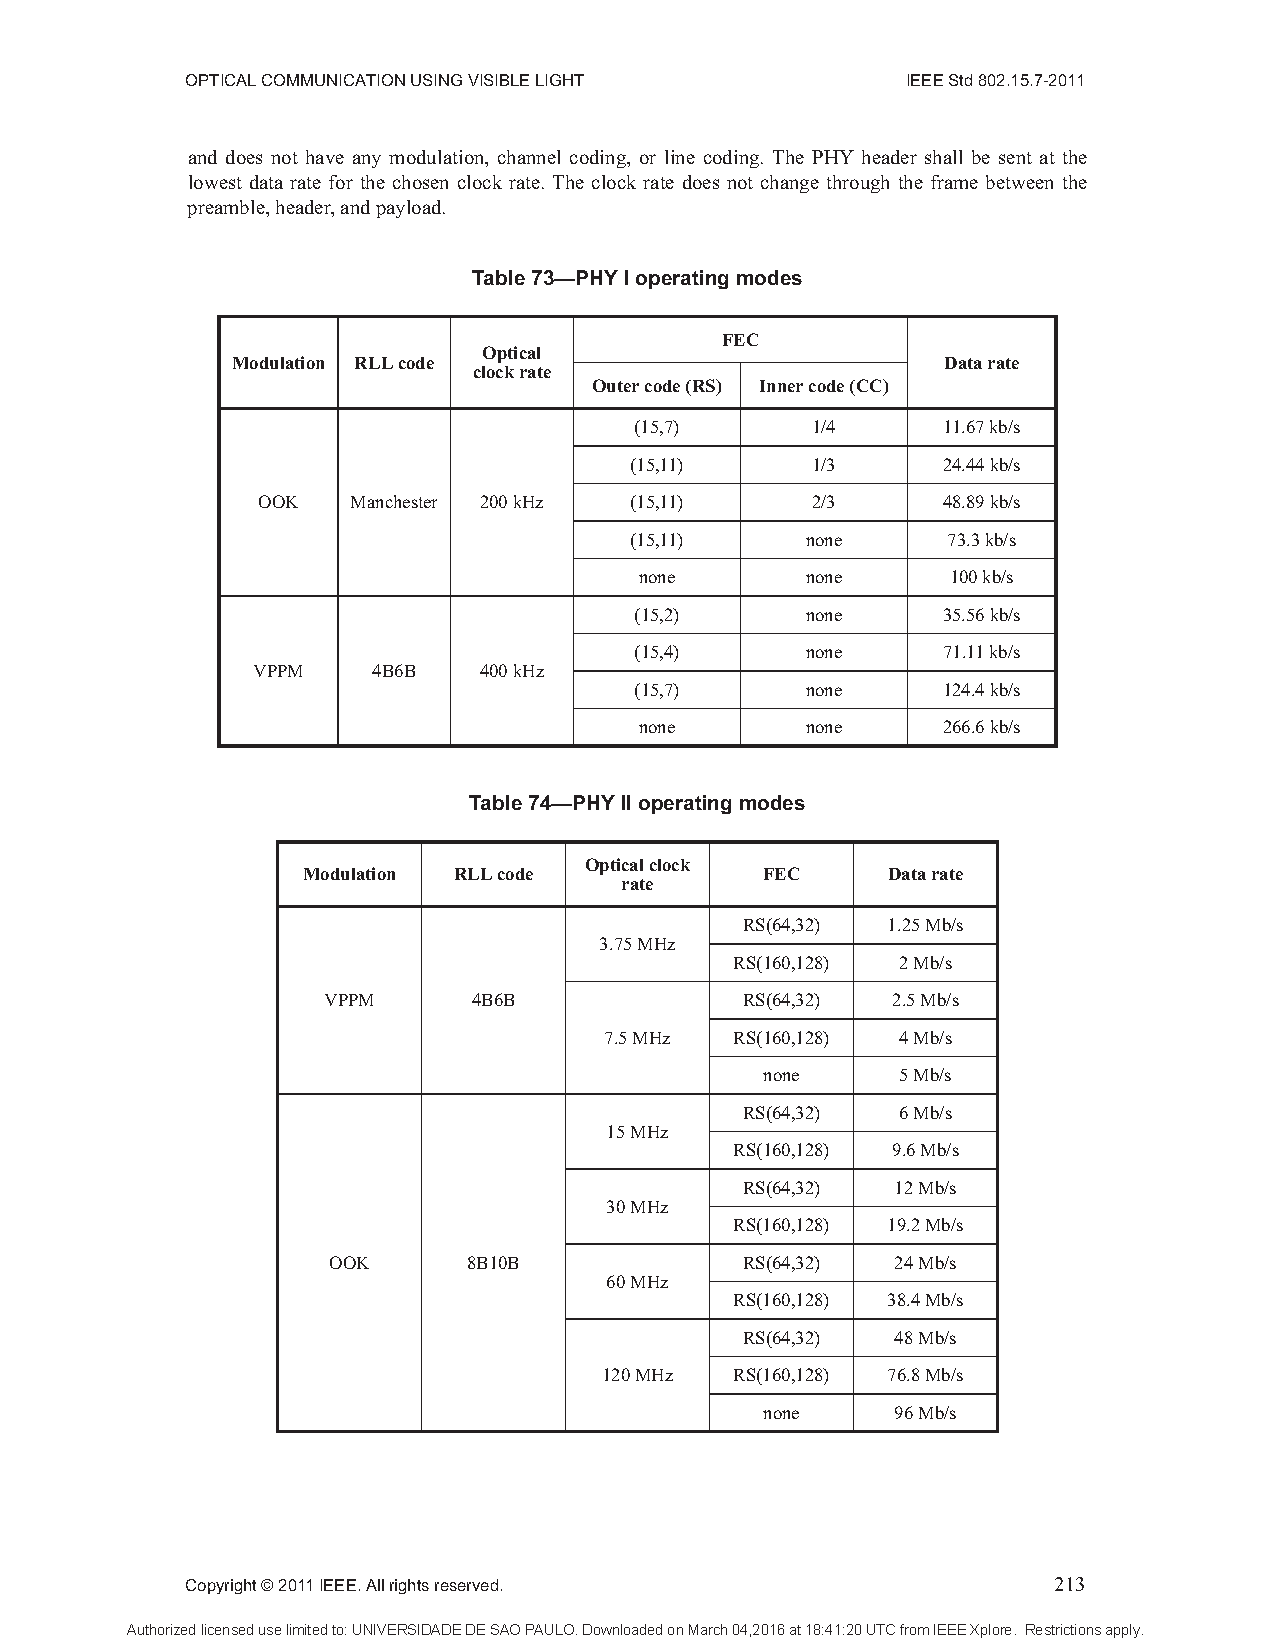
\includegraphics[clip, trim=37mm 151mm 36mm 51mm,  width=0.7\textwidth]{pag213.pdf}
		\legend{Fonte: IEEE 802.15.7}
	\end{table}
	
	\begin{table}[htbp]
		\caption{\label{tab_phy2} Modos de operação da camada PHY II de Li-Fi}
		\centering
			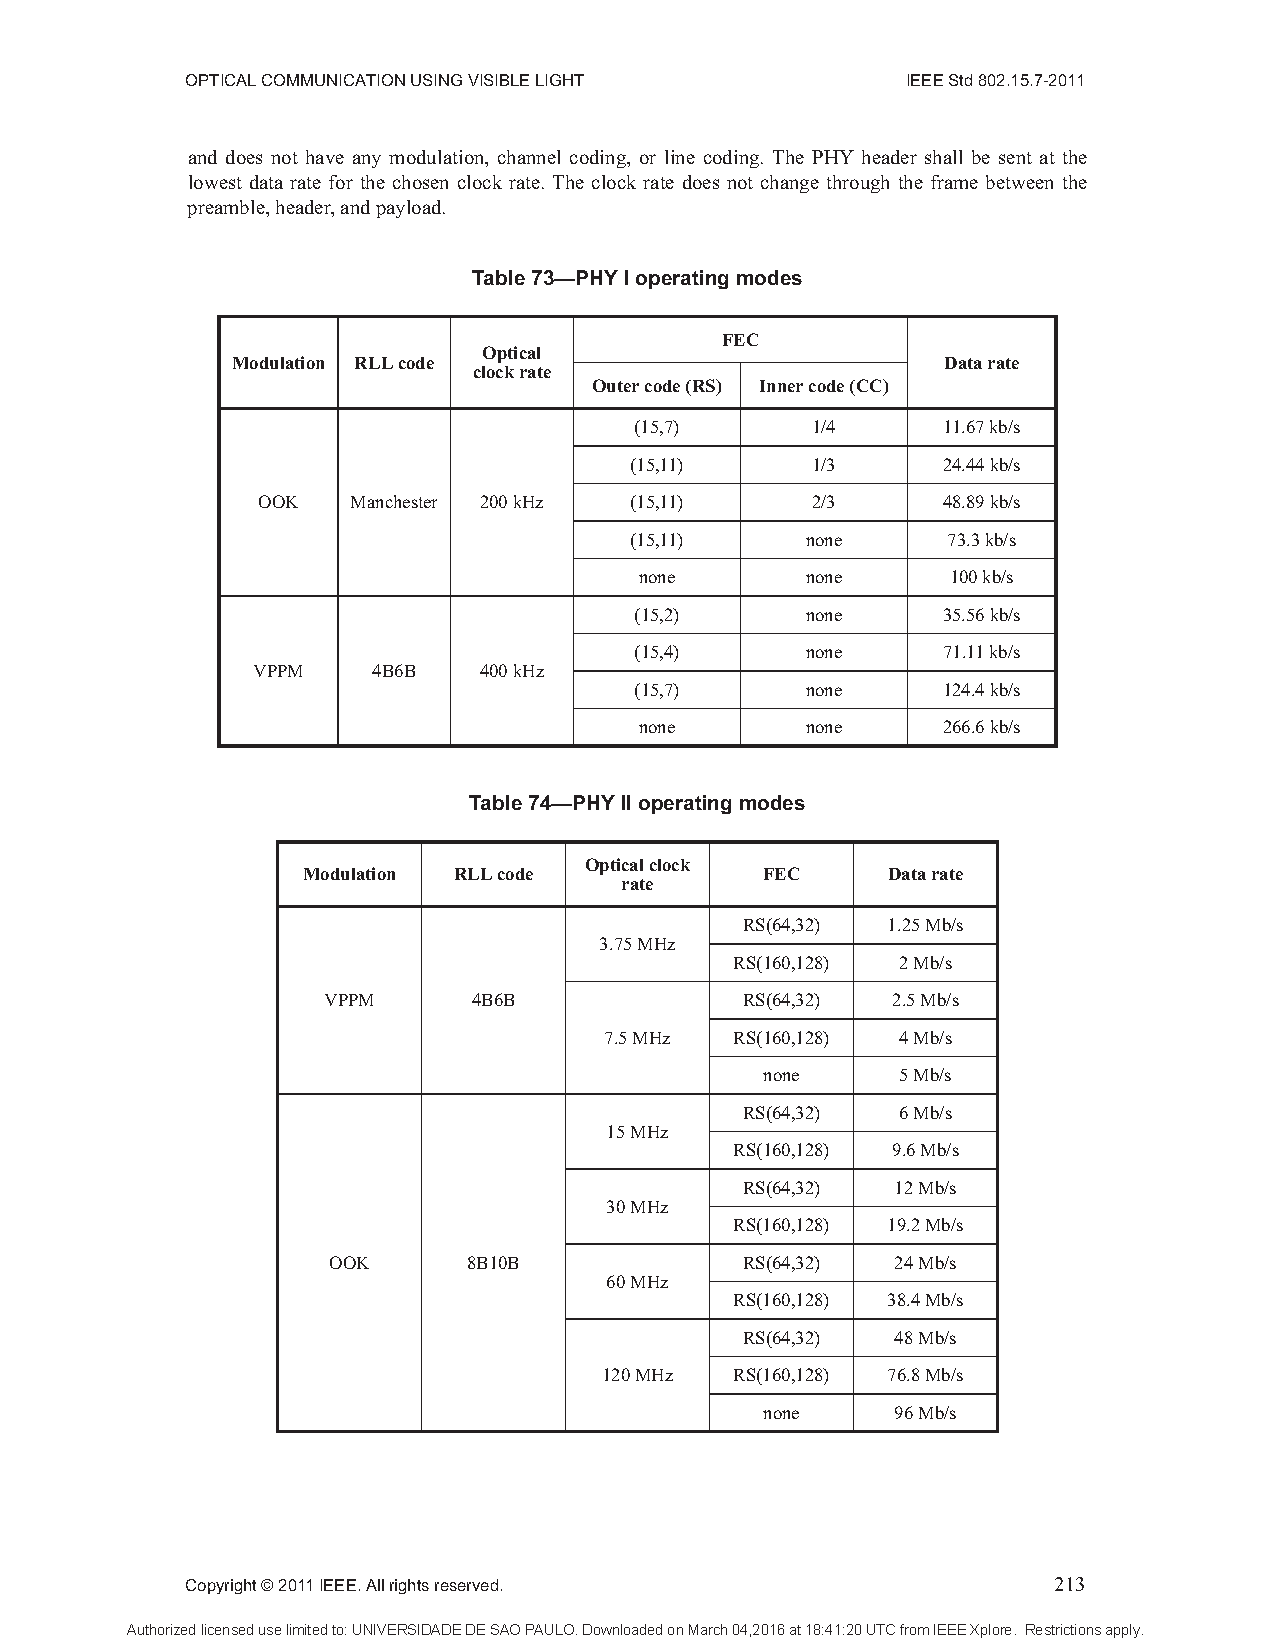
\includegraphics[clip, trim=46.55mm 36.79mm 46.74mm 142.30mm,  width=0.7\textwidth]{pag213.pdf}
		\legend{Fonte: IEEE 802.15.7}
	\end{table}

	Essa tecnologia é ideal para criar protótipos de circuitos digitais. Existe neste caso a facilidade de mudar o arranjo de componentes e vias de dados, bem como a possibilidade de simulá-los e depurá-los antes mesmo de gravar as configurações no hardware. Estes são elementos chave para a criação de um ambiente controlado, para testar as funcionalidades do produto desenvolvido. Sendo assim, um dos fatores que mais motivou a escolha dessa tecnologia neste projeto.
	
	O projeto de uma FPGA possui características que anteriormente estavam associadas a sistemas baseados em processadores. Uma delas é o uso de ferramentas e interfaces de alto nível, usando diagramas de bloco representando comportamentos e linguagens de descrição de hardware (na sigla em inglês, HDL), que no entanto diferem em muito de linguagens de programação como C. 
	
	A principal vantagem do uso de uma FPGA em relação a microcontroladores está na independência das operações de processamento, que por estarem em circuitos paralelos não precisam dividir recursos, como um mesmo núcleo por exemplo. Entretanto, o alto grau de paralelismo pode resultar em maiores desafios como garantir o sincronismo e lidar com inconsistência de dados no nível de circuito. Ainda assim, é preferível neste projeto lidar com esses desafios para se beneficiar do ganho em latência e vazão de dados.
	
	% ---
	\subsubsection{Opções Consideradas}\label{fpga-options}
	% ---
	
	Explicação de quais foram as opções consideradas.
	
	% ---
	\subsubsection{Tabela Comparativa}\label{fpga-table}
	% ---
	
	Tabela de opções consideradas.
	
	% ---
	\subsection{Microcontrolador}\label{hard-uc}
	% ---
	
	O microcontrolador escolhido foi o Photon.
	
	\begin{figure}[htb]
		\caption{\label{fig_photon} Desenho esquemático do microcontrolador Photon}
		\begin{center}
			%  trim={<left> <lower> <right> <upper>} 
			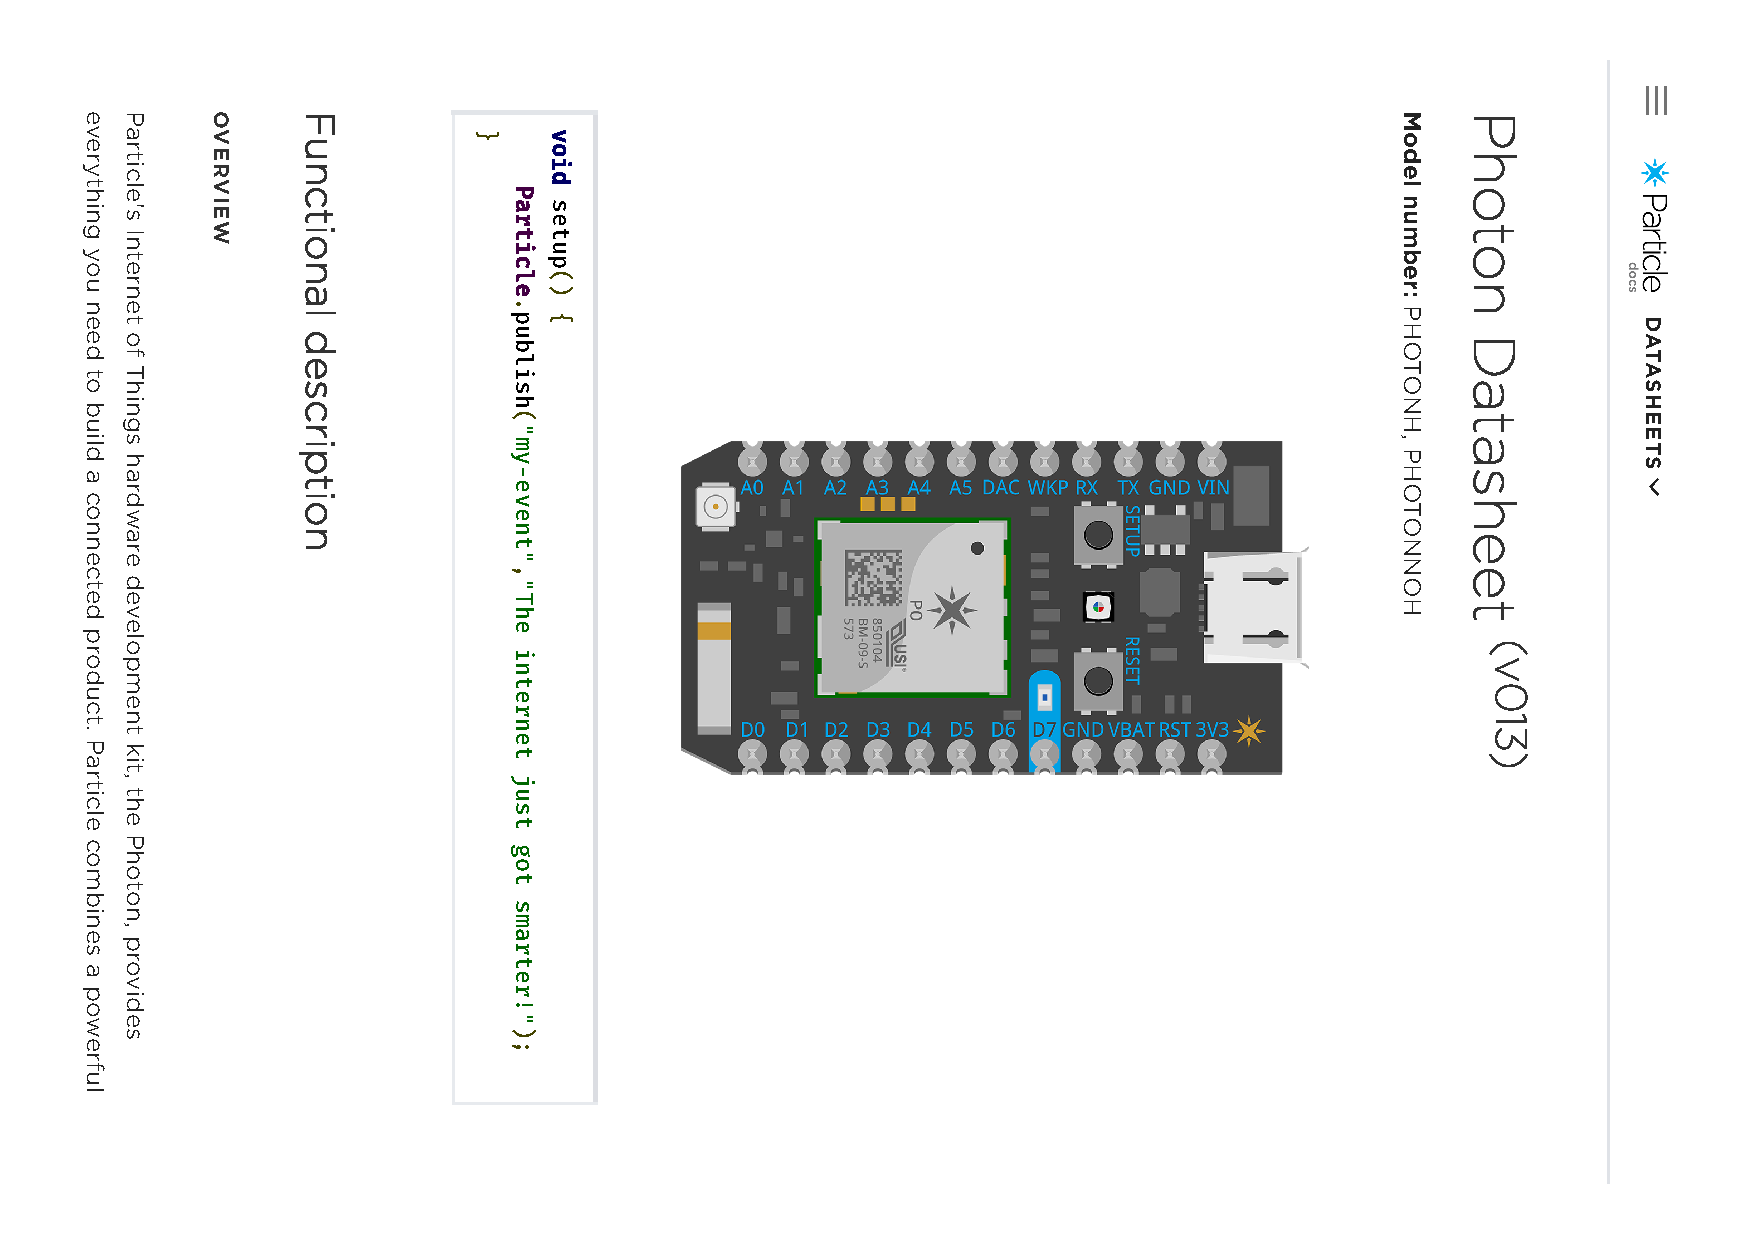
\includegraphics[width=0.5\textheight, trim={11.7cm 7.9cm 7.8cm 7.4cm}, clip]{photon.pdf}
		\end{center}
		\legend{Fonte: Particle Docs}
	\end{figure}

	
	Explicação do porquê foi escolhido microcontrolador
	
	Conexão com fgpa e microcontrolador
	The best way to connect them is to use an MCU with an external address and data bus. Then you can simply memory map the FPGA circuits into the MCU, and add your own "registers" that each have their own address. Now the FPGA can add custom peripherals, like a 32-bit timer that can latch all 4 bytes at once when the first byte is read to prevent overflows between 8-bit reads. You can also use it as glue logic to memory map more peripherals from other chips, like a separate ADC.
	
	
	% ---
	\subsubsection{Opções Consideradas}\label{uc-options}
	% ---
	
	\lipsum[14]
	
	% ---
	\subsubsection{Tabela Comparativa}\label{uc-table}
	% ---
	
	\lipsum[15]
	
	% ---
	\subsection{LED}\label{hard-led}
	% ---
	
	De acordo com a \autoref{tab_phy1} e \autoref{tab_phy2}, para cada camada física implementada é necessário suportar uma frequência de oscilação luminosa mínima:
	
	\begin{itemize}
		\item PHY I: 400kHz
		\item PHY II: 120MHz
	\end{itemize} 
	
	O LED escolhido para a transmissão deverá então suportar essas frequências de acordo com a implementação de cada camada. 
	
	O componente \texttt{LW-G6SP} foi escolhido.
	
	A \autoref{fig_ledpulse} define a frequência máxima de oscilação para cada corrente fornecida em seus terminais. Utilizando as informações contidas nele, será possível calcular qual corrente mais adequada para o pulso desejado:
	
	\begin{equation} \label{eq:5}
		f = 1 / T
	\end{equation}
	
	\begin{equation}
	200kHz = 1 / T
	\end{equation}
	
	
	
	
	\begin{figure}[htb]
		\caption{\label{fig_ledpulse} Gráfico do tempo do pulso luminoso em função da corrente para o LED \texttt{LW-G6SP}.}
		\begin{center}
			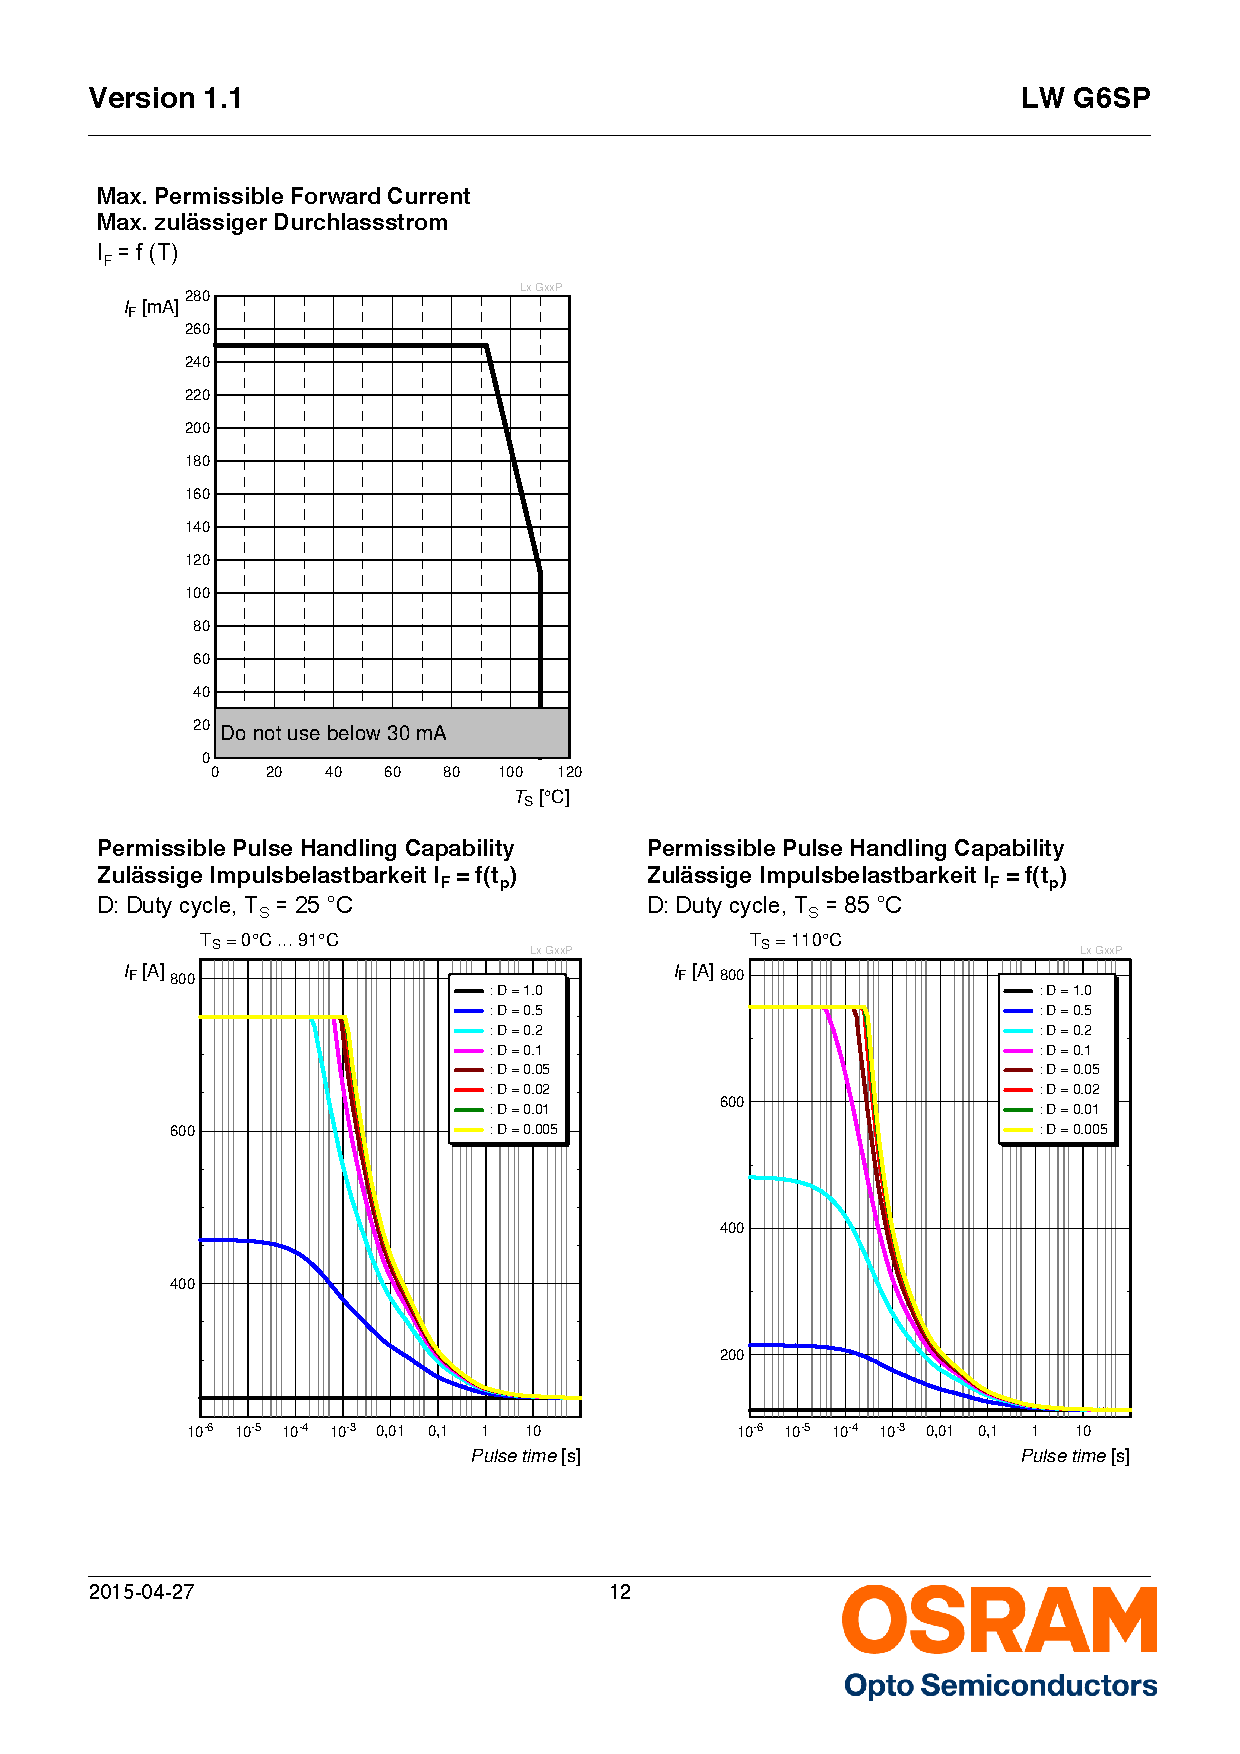
\includegraphics[width=0.3\textheight, trim={2.1cm 4.9cm 10.6cm 15.7cm}, clip]{lw-g6sp-pulse.pdf}
		\end{center}
		\legend{Fonte: OSRAM LW-G6SP Datasheet: Advanced Power TOPLED, p. 12}
	\end{figure}
	
	% ---
	\subsection{Fotodiodo}\label{hard-photodiode}
	% ---
	
	O fotodiodo é o componente 
	
	
	% ---
	\subsection{Circuito de Amplificação}\label{hard-opamp}
	% ---
	
	Com intuito de reduzir o ruido da luz ambiente, o circuito passa-faixas amplificador a seguir (\autoref{fig_opampdif}) foi proposto para o projeto:
	
	\begin{figure}[htb]
		\caption{\label{fig_opampdif}Circuito amplificador de diferenças.}
		\centering
		%  trim={<left> <lower> <right> <upper>} 
		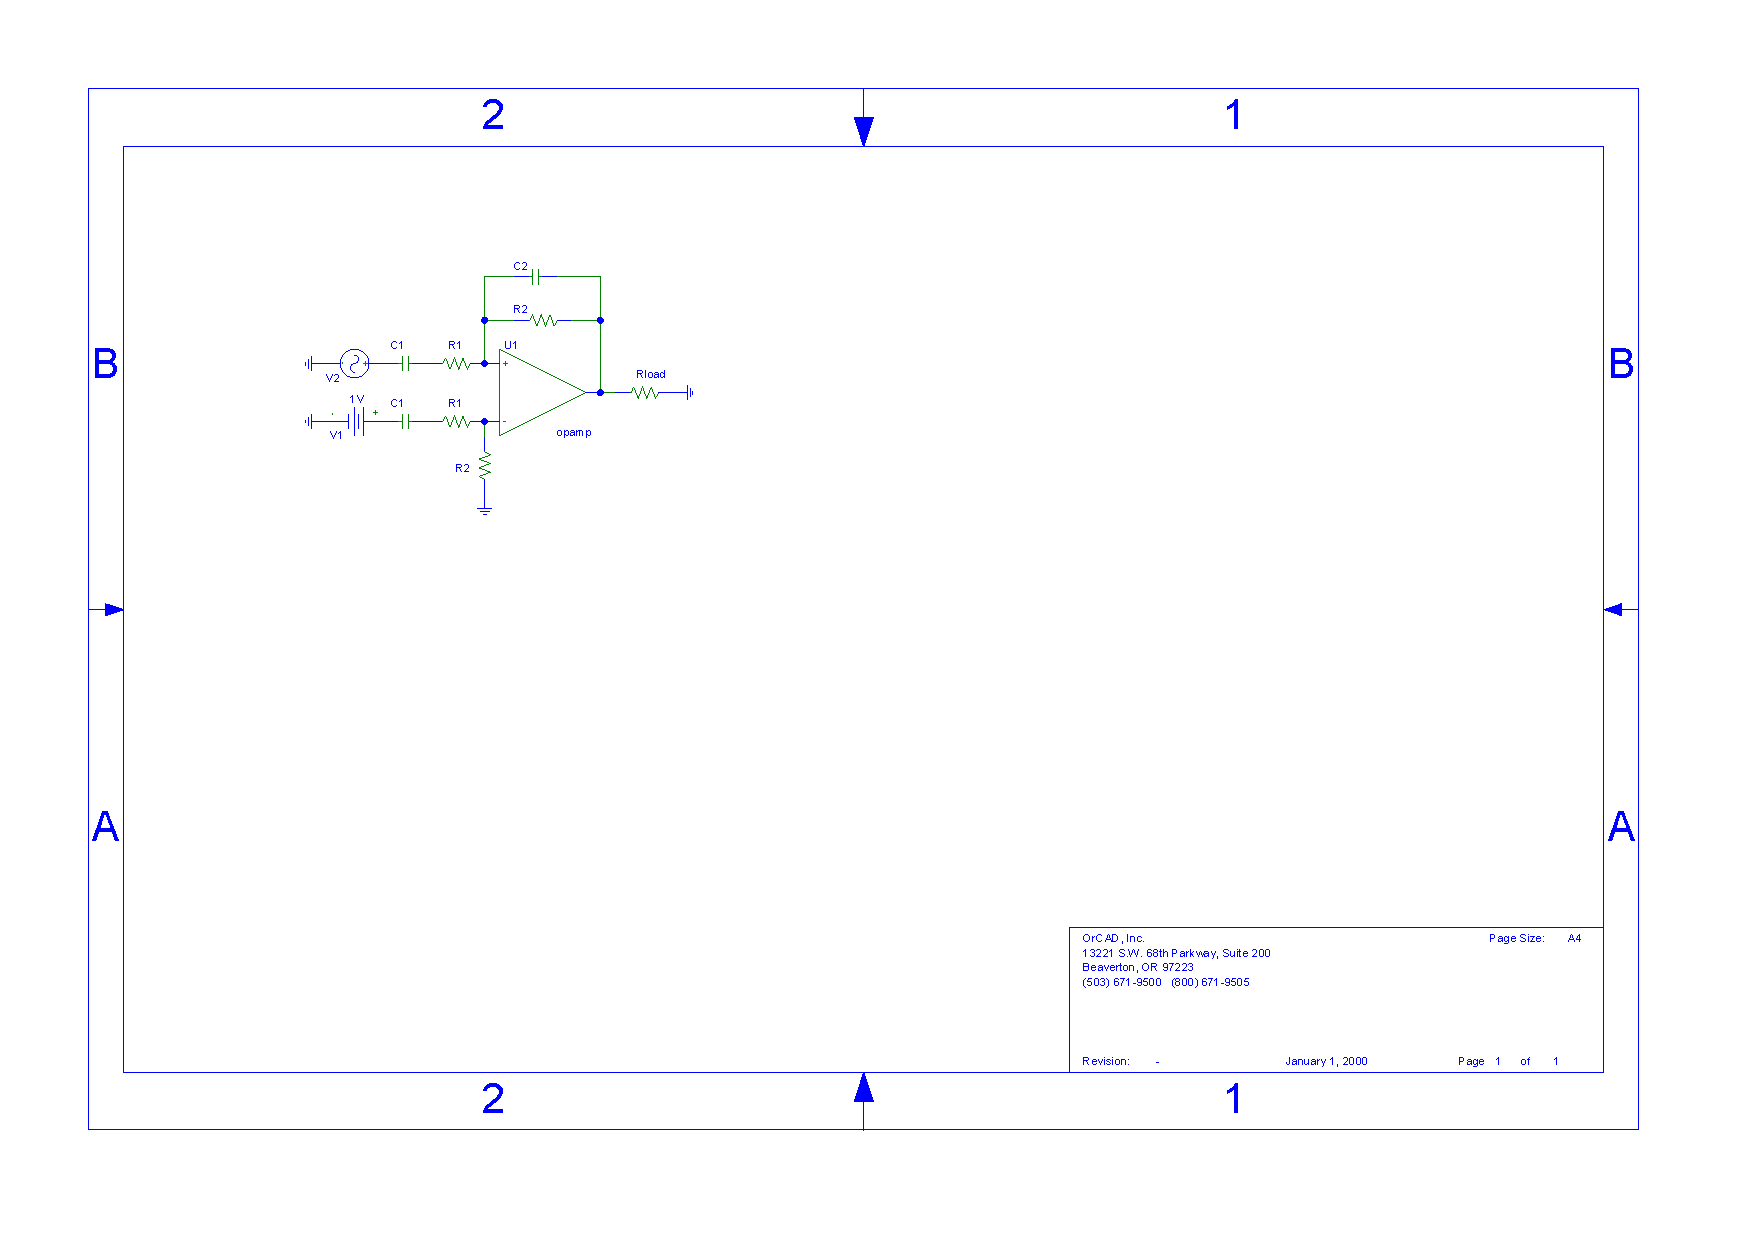
\includegraphics[width=0.6\textwidth, trim={5cm 12.29cm 17.6cm 4.3cm},clip]{opamp-dif2.pdf}
		%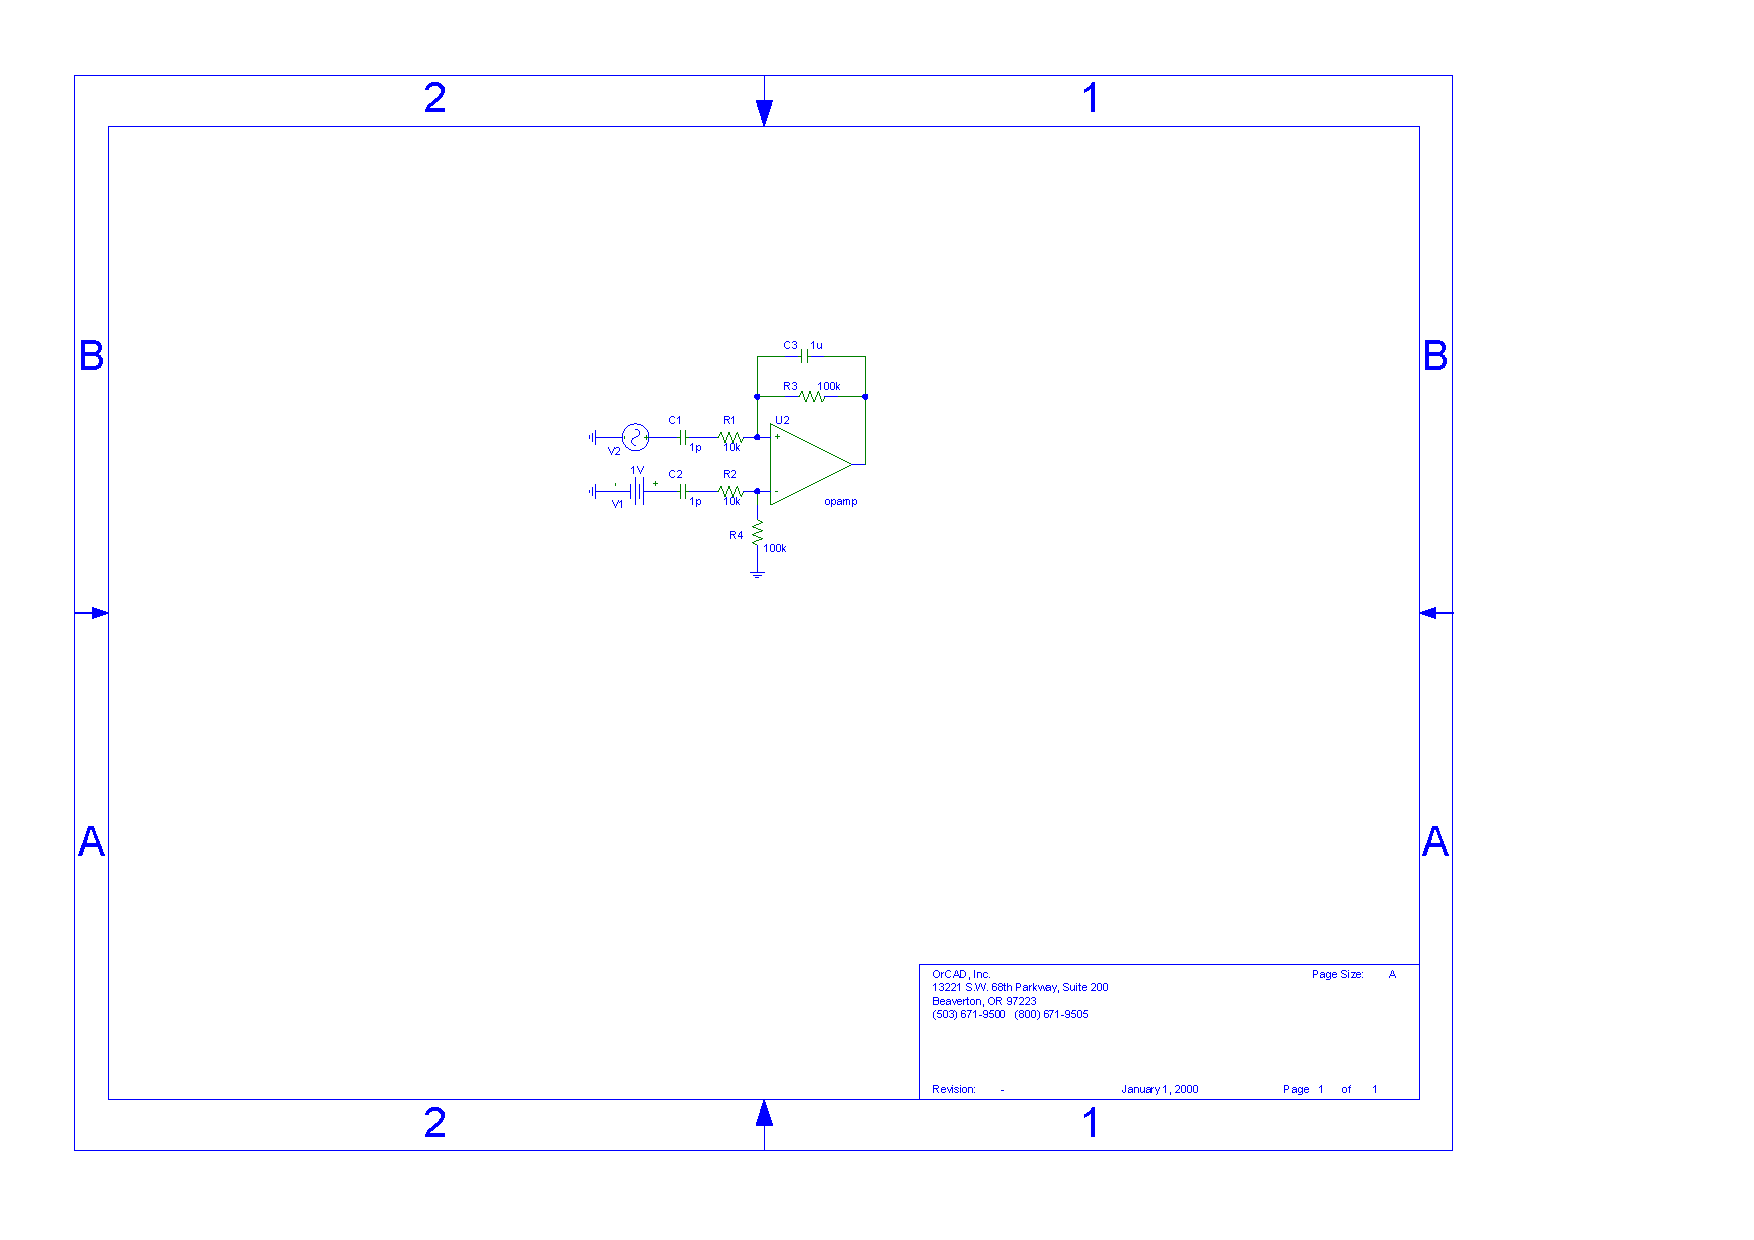
\includegraphics[width=0.5\textwidth, trim={9.5cm 11.2cm 15cm %5.76cm},clip]{opamp-dif.pdf}
		\legend{Fonte: Próprios autores}
	\end{figure}
	
	De acordo com as tabelas \ref{tab_phy1} e \ref{tab_phy2}, o intervalo da frequência do \textit{clock} luminoso é de 200kHz até 120MHz. Deseja-se então  permitir a passagem dessas, limitando as frequências fora desse intervalo. Com o uso do passa baixas e passa altas da figura acima, pode-se realizar essa limitação adequando os resistores e capacitores do circuito.
	
	\begin{figure}[htb]
		\caption{\label{fig_frequenciacentral}Um gráfico em escala logaritmica mostrando a banda de passagem B, a frequência de corte inferior Fl, a frequência de corte superior Fh e a frequência central fo para um circuito passa faixas.}
		\centering
		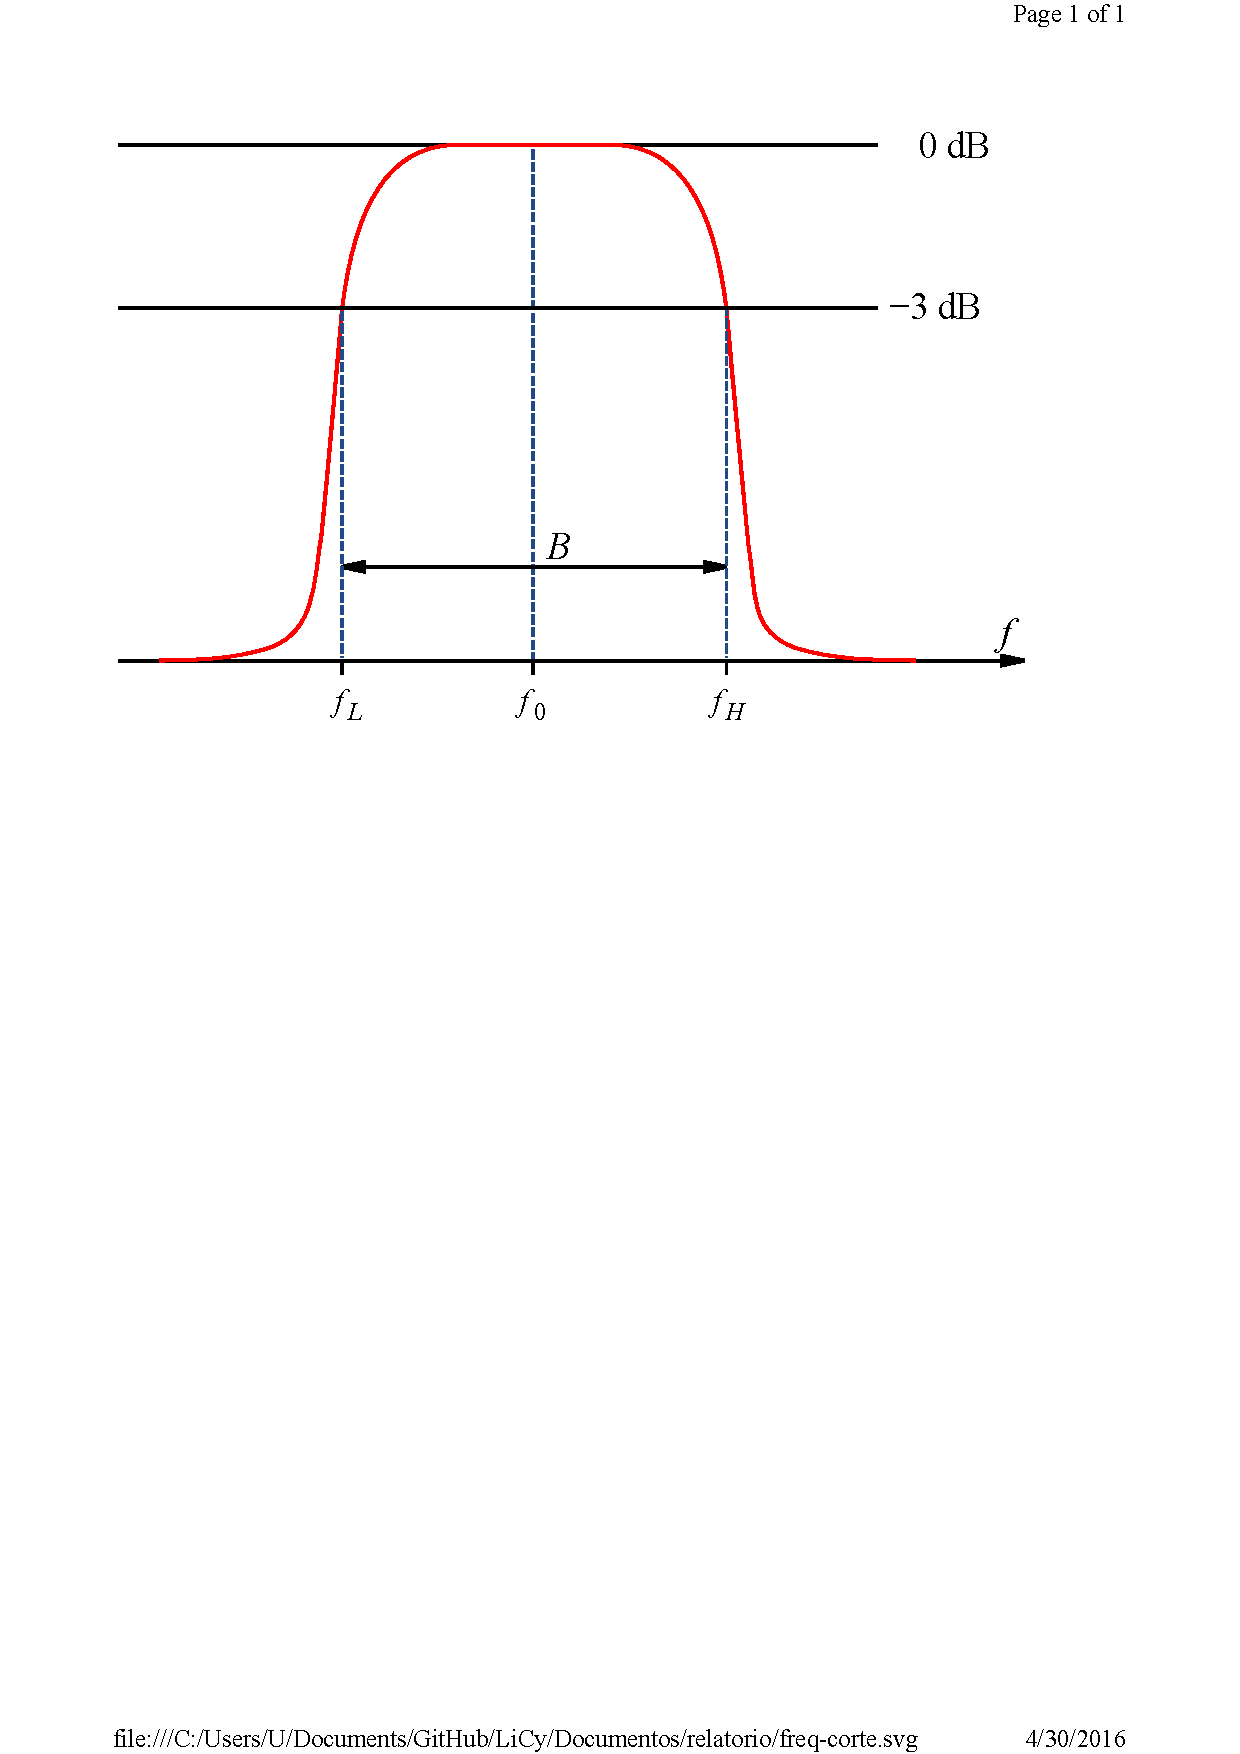
\includegraphics[width=0.5\textwidth, trim={4.5cm 17cm 3.3cm 2cm},clip]{freq-corte.pdf}
		\legend{Fonte: Inductiveload, Wikipedia}
	\end{figure}
	
	Deve-se levar em conta também o ganho do circuito, que é dado pela fórmula:
	
	\begin{equation}
		V_{out} = V_{in} \cdot \frac{R2}{R1}
	\end{equation}
	
	O cálculo da frequência de corte inferior do circuito é dado por: 
	
	\begin{equation} \label{eq:1}
		f_{ci} = \frac{1}{2 \cdot \pi \cdot R1 \cdot C1}
	\end{equation}
	
	No caso da frequência de corte superior, pode-se realizar o cálculo utilizando a fórmula abaixo:
	
	\begin{equation} \label{eq:2}
		f_{ci} = \frac{1}{2 \cdot \pi \cdot R2 \cdot C2}
	\end{equation}
	
	O cálculo da frequência central é feita pela \texttt{média geométrica} das frequências calculadas em \ref{eq:1} and \ref{eq:2} abaixo: 
	
	\begin{equation} \label{eq:3}
		f_{o} = \sqrt{f_{ci} \cdot f_{cs}}
	\end{equation}
	
	\begin{equation} \label{eq:4}
		BW = f_{ci} - f_{cs}
	\end{equation}
	
	Explicação de porque foi escolhido o circuito com ampop em modo diferencial para o projeto.
	
	% ---
	\section{Software}\label{sec-software}
	% ---
	
	Explica as escolhas feitas no aspecto do software do projeto.
	
	% ---
	\subsection{VHDL}\label{soft-vhdl}
	% ---
	
	Explicação do porquê foi escolhido VHDL
	
	% ---
	\subsubsection{Opções Consideradas}\label{vhdl-options}
	% ---
	
	Explicação de quais foram as opções consideradas.
	
	% ---
	\subsubsection{Tabela Comparativa}\label{vhdl-table}
	% ---
	
	Tabela de opções consideradas.
	
	% ---
	\subsection{Quartus}\label{soft-quartus}
	% ---
	
	Explicação do porquê foi escolhido Quartus
	
	% ---
	\subsubsection{Opções Consideradas}\label{quartus-options}
	% ---
	
	\lipsum[10]
	
	% ---
	\subsubsection{Tabela Comparativa}\label{quartus-table}
	% ---
	
	\lipsum[11]
	
	% ---
	\subsection{Android}\label{soft-android}
	% ---
	
	Explicação do porquê foi escolhido Android.
